\chapter{Data Analysis}
As mentioned before, though of fast flipping and tremendous effort to keep electron beam in exactly
the same conditions (intensity, energy, position and angle on target) through 
opposite helicity states, life is not easy and there is no way to achieve such
a goal, after all, no one can understand completely and control every aspect of
something as complicated as an accelerator. There is always various noise caused
in various parts of the machine, though very small in general sense, they are
large compare to what we want to measure, and actually the largest correction
to PV asymmetry. So we need to remove such noise in the raw asymmetry we measured.

We use the same methods to process both PREX-II and CREX data, therefore we will
talk about only CREX data here.

CREX started commissioning around December 2019, we took the first good run on 
Dec 12. 6 slugs (slug 100 - 105) were collected before the Christmas. After 
the Christmas break, data taking was resumed until Jan 18 2020 when the \Ca 
target was damaged accidently. It tooks 5 days to prepare a new \Ca target.
Things moving on quite smoothly, we had 2 days of transverse asymmetry 
measurement from Feb 10 to Feb 12. We were a little over halfway on data taking 
when Covid-19 hitted and the lab was shut down at the end of March 2020. Fortunately,
things came back 4 months later, we had the chance to continue data taking for
about 1 month. The experiment stopped data taking on Sep 18 2020. A total charge
of 480 C was collected, among which 380 C was good charge. The dataset was clearly
seperated into 3 parts: before AT, after AT (before Covid) and after Covid, which
we will talk about later.
\begin{figure}[h!]
    \begin{tikzpicture}
	\begin{scope}
	    \node[anchor=south west, inner sep=0] (image) at (0, 0)
	    {   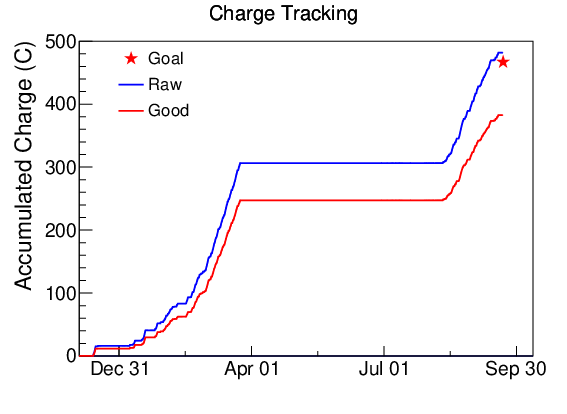
\includegraphics[width=0.45\linewidth]{charge_vs_time}
		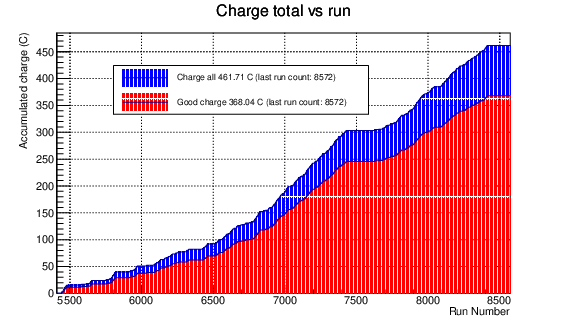
\includegraphics[width=0.54\linewidth]{charge_vs_run} };
	    \begin{scope}[x={(image.south east)},y={(image.north west)}]
		\node [Violet] at (0.3, 0.8) {Covid-shutdown};
		\draw [-stealth, Violet, line width=1pt] (0.3, 0.8) -- (0.3, 0.6);
		\node [Violet] at (0.2, 0.65) {AT};
		\draw [-stealth, Violet, line width=1pt] (0.2, 0.65) -- (0.2, 0.3);
	    \end{scope}
	\end{scope}
    \end{tikzpicture}
    \caption{Charge accumulation versus time (left) and run number (right). The
    long plateau on the left plot is due to Covid shutdown, which is shown around
    run 7500 on the right plot. We see that data taking is most efficient after
    AT (before Covid), the last month (after Covid) is not bad while the 
    first 2 months is not so efficient due to various problems.}
\end{figure}

\begin{itemize}
    \item non-linearity from electronics read out: false asymmetry. PMT $\rightarrow$
	preamplifier $\rightarrow$ ADC
\end{itemize}

Data quality:
\begin{itemize}
    \item Beam excursion: data quality cuts are applied to remove unstable beam periods
	FIXME: a plot for beam excursion
\end{itemize}

%%%%%%%%%%%%%%%%%%%%%%%%%%%%%%%%%%%%%%%%%%%%%%%%%%%%%%%%%%%%%%%%%%%%%%%%
\section{Raw Data}
What we call one event is all electrons counted in one helicity window.
The asymmetry value is calculated using every 4 (8 in PREX-II) helicity windows
(+\-\-+ or -++-)to cancel the 60 Hz line power noise. The helicity pattern was
chosed pseduo-randomly. The CREX data consists of ??? event.

beam jetter ??? in position, ??? in energy and ??? in time scale

Every event
is accompanied by a set of beam parameter values, recording the beam conditions
in that helicity window. A series of cut will be applied, basing on the beam
stability, to select good charge.

\subsubsection{Pair value}
For any 2 continuous events, define their pair value as:
For BPM/BCM, the pair difference is:
$$ diff = \frac{v^+ - v^-}{2} $$

For usl/usr, the asymmetry is:
$$ asym = \frac{v^+ - v^-}{v^+ + v^-} $$

\subsection{Measured Asymmetry}
\subsection{Beam False Asymmetry}

%%%%%%%%%%%%%%%%%%%%%%%%%%%%%%%%%%%%%%%%%%%%%%%%%%%%%%%%%%%%%%%%%%%%%%%%
\section{Regression}
\subsection{The Model}
Considering one monitor and one detector. Assuming the reading noise of both 
monitors and detectors follow the Gaussian distribution:
\begin{equation*}
    \begin{gathered}
	M = m + \epsilon(0, \sigma_0^M)    \\
	D = d + \epsilon(0, \sigma_0^D)    \\
    \end{gathered}
\end{equation*}
Here, M (D) is the measured value while m (d) is the real value and
$\sigma_0^M$ ($\sigma_0^D$) is the variance of the noise for Monitor (Detector).

Then the difference between beams of opposite polarization will follow also
the Gaussian distribution with a larger variance:
\begin{equation*}
    \begin{gathered}
	\Delta M = M^+ - M^- = (m^+ + \epsilon(0, \sigma_0^M)) - (m^- + \epsilon(0, \sigma_0^M))
	    = \Delta m_0 + \epsilon(0, \sqrt{2}\sigma_0^M)
	    = \Delta m_0 + \epsilon(0, \sigma_1^M) \\
	\Delta D = D^+ - D^- = (d^+ + \epsilon(0, \sigma_0^D)) - (d^- + \epsilon(0, \sigma_0^D))
	    = \Delta d_0 + \epsilon(0, \sqrt{2}\sigma_0^D)
	    = \Delta d_0 + \epsilon(0, \sigma_1^D) \\
    \end{gathered}
\end{equation*}
Again, $(\Delta M)_0$ ($\Delta D)_0$ is the real difference between the
different polarized beam while $\Delta M$ ($\Delta D$) is the measured value.

The probability for measuring $\Delta M$ and $\Delta D$ will be:
\begin{equation*}
    \begin{gathered}
	P(\Delta M) = \frac{1}{\sigma_1^M\sqrt{2\pi}} e^{-\frac{1}{2}\left( \frac{\Delta M - \Delta m_0}{\sigma_1^M}\right)^2}    \\
	P(\Delta D) = \frac{1}{\sigma_1^D\sqrt{2\pi}} e^{-\frac{1}{2}\left( \frac{\Delta D - \Delta d_0}{\sigma_1^D}\right)^2}    \\
    \end{gathered}
\end{equation*}

We will have a bunch of data points: $(\Delta M, \Delta D)_i$ and we want to
extract the relationship between $\Delta d_0$ and $\Delta m_0$: $c \equiv \frac{\partial D}{\partial M}$,
we will use regression to derive it (assuming linear relationship).
$$ \Delta d = c \Delta m $$

For any real data point $(\Delta m_0, \Delta d_0)_i$, the possibility to measure
$(\Delta M, \Delta D)_i$ is:
\begin{equation*}
    \begin{gathered}
	P_i(\Delta D|\Delta M) = \frac{1}{\sigma_1^D\sqrt{2\pi}} 
	    e^{-\frac{1}{2}\left( \frac{\Delta D - c\Delta m_0}{\sigma_1^D}\right)^2}
    \end{gathered}
\end{equation*}

For the accumulated data of one minirun (about 5 mins of data taking), the total
probability will be:
\begin{equation*}
    P = \prod_i^n P_i(\Delta D|\Delta M) = \prod_i^n \frac{1}{\sigma_1^D\sqrt{2\pi}} 
	    e^{-\frac{1}{2}\left( \frac{\Delta D_i - c\Delta m_0}{\sigma_1^D}\right)^2}
\end{equation*}



%%%%%%%%%%%%%%%%%%%%%%%%%%%%%%%%%%%%%%%%%%%%%%%%%%%%%%%%%%%%%%%%%%%%%%%%
\section{Beam Modulation}

%%%%%%%%%%%%%%%%%%%%%%%%%%%%%%%%%%%%%%%%%%%%%%%%%%%%%%%%%%%%%%%%%%%%%%%%
\section{Lagragian}

%%%%%%%%%%%%%%%%%%%%%%%%%%%%%%%%%%%%%%%%%%%%%%%%%%%%%%%%%%%%%%%%%%%%%%%%
\section{Correction}
\begin{itemize}
    \item background dilution
\end{itemize}
%%%%%%%%%%%%%%%%%%%%%%%%%%%%%%%%%%%%%%%%%%%%%%%%%%%%%%%%%%%%%%%%%%%%%%%%
\section{Result}
